\documentclass[tikz,border=8pt]{standalone}
\usepackage{lmodern}
\usetikzlibrary{arrows.meta,calc,decorations.pathreplacing}
\definecolor{ink}{HTML}{183B4E}
\definecolor{teal}{HTML}{168C8C}
\definecolor{gold}{HTML}{D9982F}
\definecolor{violet}{HTML}{7B61A8}
\definecolor{softblue}{HTML}{EAF4F6}
\definecolor{softgold}{HTML}{FFF4D8}
\begin{document}
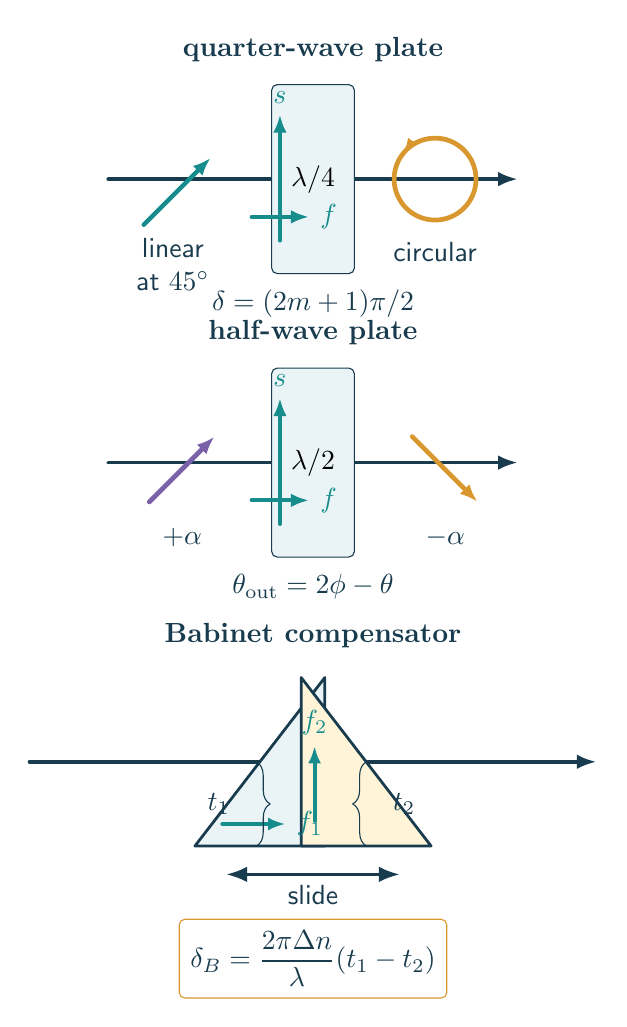
\begin{tikzpicture}[>=Latex,line cap=round,line join=round,font=\sffamily]
  \tikzset{
    plate/.style={draw=ink,fill=softblue,rounded corners=2pt,minimum width=1.05cm,minimum height=2.4cm},
    beam/.style={ink,line width=1.35pt,-{Latex[length=2.5mm]}},
    axisarrow/.style={teal,line width=1.45pt,-{Latex[length=2.3mm]}}
  }

  % Quarter-wave plate.
  \begin{scope}[shift={(1.0,7.35)}]
    \node[ink,font=\bfseries] at (2.5,2.85) {quarter-wave plate};
    \draw[beam] (-0.1,1.2)--(5.1,1.2);
    \node[plate] (Q) at (2.5,1.2) {$\lambda/4$};
    \draw[axisarrow] (2.08,0.42)--(2.08,2.02) node[above] {$s$};
    \draw[axisarrow] (1.72,0.72)--(2.45,0.72) node[right] {$f$};
    \draw[teal,line width=1.6pt,-{Latex[length=2.3mm]}] (0.35,0.62)--(1.20,1.47);
    \node[ink,align=center] at (0.72,0.12) {linear\\at $45^\circ$};
    \draw[gold,line width=1.7pt] (4.05,1.2) circle (0.52);
    \draw[gold,-{Latex[length=2mm]},line width=1.4pt] (4.42,1.57) arc[start angle=45,end angle=142,radius=.52];
    \node[ink] at (4.05,0.28) {circular};
    \node[ink] at (2.5,-0.38) {$\delta=(2m+1)\pi/2$};
  \end{scope}

  % Half-wave plate.
  \begin{scope}[shift={(1.0,3.75)}]
    \node[ink,font=\bfseries] at (2.5,2.85) {half-wave plate};
    \draw[beam] (-0.1,1.2)--(5.1,1.2);
    \node[plate] (H) at (2.5,1.2) {$\lambda/2$};
    \draw[axisarrow] (2.08,0.42)--(2.08,2.02) node[above] {$s$};
    \draw[axisarrow] (1.72,0.72)--(2.45,0.72) node[right] {$f$};
    \draw[violet,line width=1.7pt,-{Latex[length=2.3mm]}] (0.42,0.70)--(1.25,1.53);
    \draw[gold,line width=1.7pt,-{Latex[length=2.3mm]}] (3.76,1.53)--(4.59,0.70);
    \node[ink] at (0.84,0.25) {$+\alpha$};
    \node[ink] at (4.18,0.25) {$-\alpha$};
    \node[ink] at (2.5,-0.38) {$\theta_{\rm out}=2\phi-\theta$};
  \end{scope}

  % Babinet compensator.
  \begin{scope}[shift={(0,-0.10)}]
    \node[ink,font=\bfseries] at (3.50,2.85) {Babinet compensator};
    \draw[beam] (-0.10,1.25)--(7.10,1.25);
    \path[draw=ink,fill=softblue,line width=1pt]
      (2.00,0.18)--(3.65,2.32)--(3.65,0.18)--cycle;
    \path[draw=ink,fill=softgold,line width=1pt]
      (3.35,2.32)--(5.00,0.18)--(3.35,0.18)--cycle;
    \draw[teal,line width=1.5pt,-{Latex[length=2.2mm]}] (2.35,0.46)--(3.15,0.46) node[right] {$f_1$};
    \draw[teal,line width=1.5pt,-{Latex[length=2.2mm]}] (3.52,0.50)--(3.52,1.45) node[above] {$f_2$};
    \draw[ink,<->,line width=1pt] (2.40,-0.18)--(4.60,-0.18) node[midway,below] {slide};
    \draw[decorate,decoration={brace,amplitude=5pt},ink]
      (2.78,1.25)--(2.78,0.18) node[midway,left=6pt] {$t_1$};
    \draw[decorate,decoration={brace,amplitude=5pt},ink]
      (4.18,0.18)--(4.18,1.25) node[midway,right=6pt] {$t_2$};
    \node[draw=gold,fill=white,rounded corners=2pt,inner sep=4pt,text=ink]
      at (3.50,-1.25)
      {$\displaystyle\delta_B=\frac{2\pi\Delta n}{\lambda}(t_1-t_2)$};
  \end{scope}
\end{tikzpicture}
\end{document}
